%-----------------------------------------------------------------------------%
\chapter{\topikEmpat}
%-----------------------------------------------------------------------------%

%-----------------------------------------------------------------------------%
\section{Pendahuluan}
%-----------------------------------------------------------------------------%

AMBER (\f{Assisted Model Building with Energy Refinement}) adalah paket program untuk menjalankan simulasi dinamika molekular (\f{molecular dynamics}) yang dikembangkan oleh \f{University of California}, San Fransico. Alamat \f{website} resmi dari AMBER adalah \url{http://ambermd.org}.

AMBER digunakan untuk berbagai eksperimen dinamika molekular seperti simulasi pergerakan fisik dari atom dan molekular, pemodelan protein dan eksperimen yang terkait dengan perancangan obat (\f{drug discovery}).

AMBER didistribusikan dalam dua bagian:

\begin{enumerate}
	\item AMBER (berbayar, versi terakhir 14)
	\item AMBERTool (\f{opensource} GPL, versi terakhir 15)
\end{enumerate}

AMBER memiliki dua mode instalasi, yaitu berbasis CPU (dengan OpenMPI) dan berbasis GPU (dengan CUDA). Petunjuk instalasi dapat dilihat di \url{http://jswails.wikidot.com/installing-amber14-and-ambertools14}.


%-----------------------------------------------------------------------------%
\section{Eksperimen}
%-----------------------------------------------------------------------------%

Percobaan dilakukan dengan menjalankan 6 buah eksperimen yang disediakan pada AMBER GPU \f{Benchmark Suite} yang diperoleh dari \f{website} resmi AMBER \url{http://ambermd.org/Amber14_Benchmark_Suite.tar.bz2}. Enam buah eksperimen yang kami jalankan adalah:

\begin{enumerate}
	\item \verb|TRPCAGE Production| (304 atoms, 250.000 nsteps)
	\item \verb|Myoglobin Production| (2,492 atoms, 25.000 nsteps)
	\item \verb|JAC Production NVE| (23,558 atoms, 25.000 nsteps)
	\item \verb|Nucleosome Production| (25,095 atoms, 600 nsteps)
	\item \verb|Factor IX Production NVE| (90,906 atoms, 10.000 nsteps)
	\item \verb|Cellulose Production NVE| (408,609 atoms, 5.000 nsteps)	
\end{enumerate}

Pada eksperimen ini kami mengamati hubungan antara jumlah atom dan nsteps dengan kecepatan proses (\verb|ns/day|). Jika kecepatan proses meningkat seiring bertambahnya prosesor (CPU) yang digunakan berarti terjadi \speedup. Sebaliknya, jika tidak terjadi pertambahan maka tidak terjadi \speedup.

\begin{figure}
	\centering
	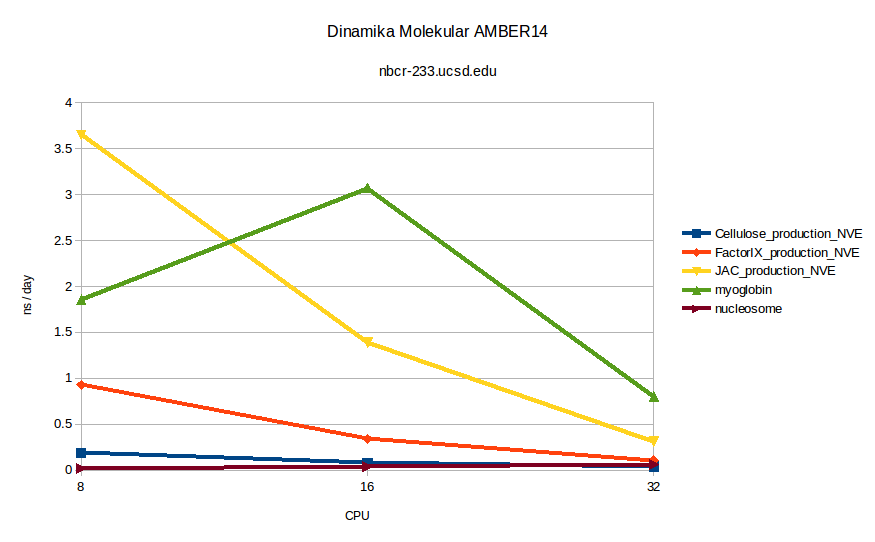
\includegraphics[width=1\textwidth]
	{pics/amber_all}
	\caption{Eksperimen AMBER di cluster UCSD}
	\label{fig:amber_all}
\end{figure}  

Hasil yang kami peroleh ditujukkan pada grafik gambar \ref{fig:amber_all}, yaitu \speedup hanya terjadi pada \verb|Cellulose_production_NVE| (CPU 8-16) dan \verb|Nucleosome|. Peningkatan kecepatan proses dapat lebih jelas lagi diamati pada gambar \ref{fig:amber_nucleosome} di mana grafik \verb|Nucleosome| dipisahkan tersendiri.

\begin{figure}
	\centering
	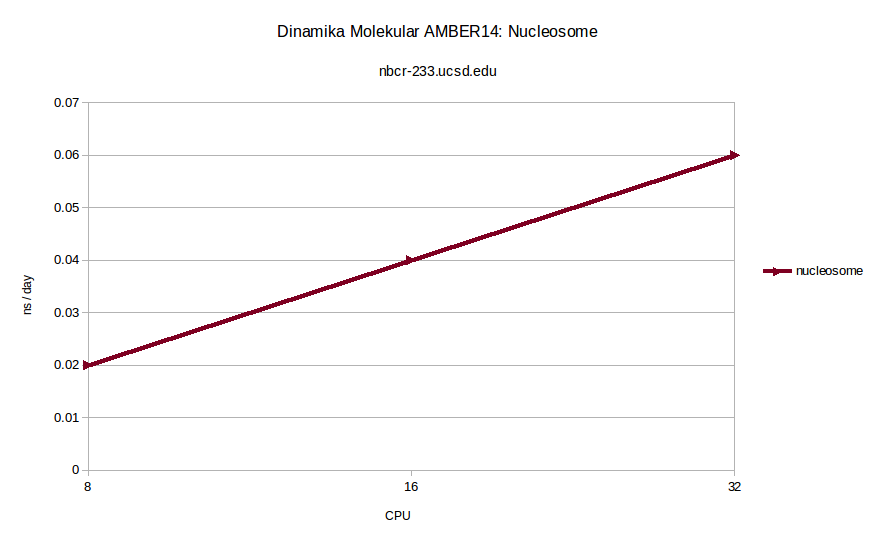
\includegraphics[width=1\textwidth]
	{pics/amber_nucleosome}
	\caption{Eksperimen AMBER Nucleosome di cluster UCSD}
	\label{fig:amber_nucleosome}
\end{figure}  


%-----------------------------------------------------------------------------%
\section{Kesimpulan}
%-----------------------------------------------------------------------------%

Berdasarkan eksperimen ini, kami menarik beberapa kesimpulan:

\begin{itemize}
	\item AMBER dapat berjalan secara paralel di atas MPI
	\item AMBER dapat melakukan prediksi kecepatan proses (dan durasi) sebelum percobaan selesai (dengan opsi \verb|mdinfo|)
	\item Kecepatan proses (\verb|ns/day|) bergantung pada jumlah atom dan nsteps
	\item Seperti halnya pada topik sebelumnya, \speedup terlihat jika proses dinamika molekuler membutuhkan banyak resource (jumlah atom besar dan nsteps kecil)
\end{itemize}